%!TEX program = xelatex

\documentclass[compress,xcolor=table]{beamer}
%--------------------------------------------------------------------------
% Common packages
%--------------------------------------------------------------------------

\definecolor{links}{HTML}{663000}
\hypersetup{colorlinks,linkcolor=,urlcolor=links}

\usepackage[english]{babel}
\usepackage{pgfpages} % required for notes on second screen
\usepackage{graphicx}

\usepackage{multicol}

\usepackage{tabularx,ragged2e}
\usepackage{booktabs}

\setlength{\emergencystretch}{3em}  % prevent overfull lines
\providecommand{\tightlist}{%
  \setlength{\itemsep}{0pt}\setlength{\parskip}{0pt}}


\usetheme{hri}

% Display the navigation bullet even without subsections
\usepackage{remreset}% tiny package containing just the \@removefromreset command
\makeatletter
\@removefromreset{subsection}{section}
\makeatother
\setcounter{subsection}{1}


\newcommand{\source}[2]{{\tiny\it Source: \href{#1}{#2}}}

\newcommand{\colvec}[2][.8]{%
  \scalebox{#1}{%
    \renewcommand{\arraystretch}{.8}%
    $\begin{bmatrix}#2\end{bmatrix}$%
  }
}


\usepackage{tikz}
\usetikzlibrary{mindmap,backgrounds,positioning,quotes,shapes}

\graphicspath{{figs/part6/}}

\title{ROCO318 \newline Mobile and Humanoid Robots}
\subtitle{Part 6 -- Localisation and Planning}

\date{}
\author{Séverin Lemaignan}
\institute{Centre for Neural Systems and Robotics\\{\bf Plymouth University}}

\begin{document}

\licenseframe{github.com/severin-lemaignan/module-mobile-and-humanoid-robots}

\maketitle

\begin{frame}{Pose and navigation}

    \textbf{Pose maintenance}

    \begin{itemize}
        \item Pose (= position and orientation) maintenance is
            keeping an as precise as possible estimate of the robot's pose.
    \end{itemize}

    \pause

    \textbf{Planning: getting from A to B}

    \begin{itemize}
        \item A cognitive skill: given partial knowledge of the environment, a
            goal and sensor readings, decide what to do to reach the goal as
            efficiently and reliably as possible.

        \item Different from inverse kinematics: IK \emph{locally} maps a
            target state (position and orientation) in a global space (\eg
            Cartesian space) to the robot's internal space (joint space, or
            generally \emph{configuration space})

        \item $\rightarrow$ IK work on a small scale (\textless{} meter) while
            planning/navigation works on larger scale (room, building, roadmap,
            \ldots{})

    \end{itemize}

\end{frame}

\begin{frame}{Planning and navigation -- traditional approach}

    Today's industrial robots can operate \textbf{without any intelligence} because
    their environment is static and very structured.

    In mobile robotics, cognition and reasoning is primarily of geometric
    nature, such as picking a safe path or determining where to go next.

    $\rightarrow$ already been largely explored in literature for cases in
    which complete information about the current situation and the environment
    exists (e.g.
    \href{http://en.wikipedia.org/wiki/Travelling_salesman_problem}{travelling
    sales man problem} or
    \href{http://en.wikipedia.org/wiki/Route_inspection_problem}{route
    inspection problem}).

\end{frame}

\begin{frame}{Kiva systems: Beacon based localisation}
    \begin{center}
        \url{http://www.youtube.com/watch?v=lWsMdN7HMuA}

        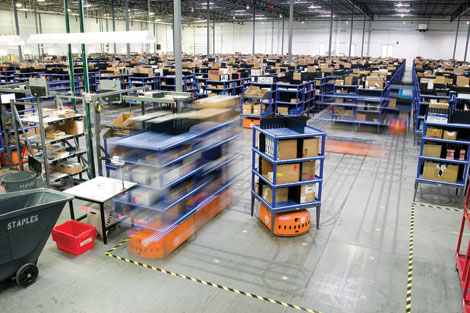
\includegraphics[width=0.8\linewidth]{kiva}
    \end{center}
\end{frame}

\section{Monte-Carlo Localisation}

\begin{frame}{Monte Carlo methods}

    \begin{columns}
        \begin{column}{0.5\linewidth}
            \textbf{Repeated random sampling to compute results}

            Used when it to difficult to calculate exact results:

            \begin{itemize}
                \item the system is complex and calculating it through is too
                    computationally expensive,
                \item or, too many variables and it is impossible to calculate all
                    possibilities (\emph{combinatorial explosion})
            \end{itemize}


        \end{column}
        \begin{column}{0.5\linewidth}
            \begin{center}
                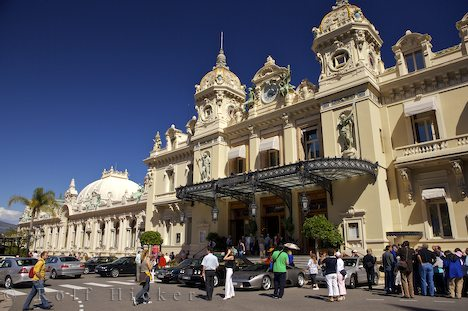
\includegraphics[width=\linewidth]{montecarlo}
            \end{center}

            \onslide<2>{
            Monte Carlo \emph{localisation} is MC methods applied to robot localisation.
            }
        \end{column}
    \end{columns}

\end{frame}

\videoframe[0.56]{figs/part6/mcl_example.mp4}

\imageframe[color=black]{localisation_pepper}

\begin{frame}{Monte-Carlo Localisation -- Introduction}

    \begin{itemize}
        \item Monte-Carlo Localisation (MCL) is a \textbf{\href{http://en.wikipedia.org/wiki/Particle_filter}{particle
            filter}}, which uses a set $S_t$ of $N$ particles at time
            $t$.
            \large
            \begin{align*}
                S_t &= \{s_t^i \quad|\quad i = 1\ldots N\} \\
                s^i &= \{\mathbf{x}^i, w^i\} \text{ with } \mathbf{x}^i =
                \colvec{x^i \\ y^i \\ \theta^i}
            \end{align*}
            \normalsize
        \item<+-> Each particle $s^i$ contains the pose of the particle $\mathbf{x}^i$ and a weight $w^i$.
        \item<+-> The sum of all weights is 1: \[ \sum_{i=1}^N w^i = 1 \]
        \item<+-> For small maps, $N$ is in the hundreds, for larger maps you
            can have thousands of particles.
    \end{itemize}

\end{frame}

\begin{frame}{Monte-Carlo Localisation -- Initialisation}

    The $N$ particles are distributed on the map

    \begin{itemize}
        \item If the robot's position is not known, they are distributed randomly
            across the map with a probability $p=\frac{1}{N}$ (\emph{uniform
            distribution}).
            \pause
        \item If the robot's position is available, the initial particle
            distribution could be Gaussian around the robot (\emph{normal
            distribution}).
    \end{itemize}

    \pause 

    Then , Monte Carlo Localisation runs through three steps:

    \begin{enumerate}
        \item Prediction phase (when the robot takes an action)
        \item Update phase (when sensor data comes in)
        \item Resampling phase
    \end{enumerate}

\end{frame}

\begin{frame}{Monte-Carlo Loclaisation - Prediction phase}

The prediction phase \textbf{essentially moves all particles} along with the
robot.

    \only<1-3>{
Example: if the robot moves 10cm right and turn 10˚ counterclockwise, then all particles are
updated:
    \Large
    \[
        s_t^i = \{ \{ x_{t-1}^i + 0.1, y_{t-1}^i, \theta_{t-1}^i - 10^{\circ}\}, w\bubblemark[0pt]{oldnochange}_{t-1}^i\}
    \]
    \normalsize

\bubble<1>[90]{oldnochange}{Note, the weight is not changed}
\pause

    This allows for a \textbf{motion model} to be implemented, by adding some noise.

    \only<2>{
    \large
    \begin{align*}
        s_t^1 &= \{ \{ x_{t-1}^1 + 0.11, y_{t-1}^1, \theta_{t-1}^1 - 10.3^{\circ}\}, w_{t-1}^1\} \\
        s_t^2 &= \{ \{ x_{t-1}^2 + 0.09, y_{t-1}^2, \theta_{t-1}^2 - 10.2^{\circ}\}, w_{t-1}^2\} \\
        ...
    \end{align*}
    \normalsize
    }

    \only<3>{
    This motion model should be based on the kinematics of your robot.
    \eg for a differential drive robot you can have a good
    idea of how imprecise it is.
    }
    }
    \only<4>{
    Formally, if the robot performs an action $a$, all $N$ particles are
    updated as follows:
        \Large
        \[ 
        \mathbf{x}_t^i =
        p(\mathbf{x}_t{}^i\bubblemark[0pt]{motionmodel}|\mathbf{x}_{t-1}{}^i, a)
        \]
    \normalsize
    \begin{columns}
        \begin{column}{0.5\linewidth}

            \vspace{1em}

        Example: repeated application of the prediction rule leads to gradual
          loss of pose accuracy:
        \end{column}
        \begin{column}{0.5\linewidth}
            \begin{center}
                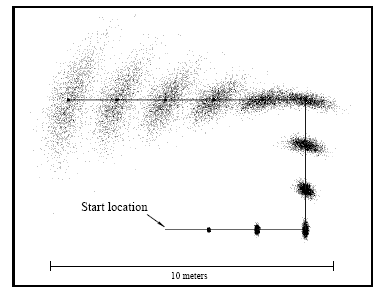
\includegraphics[width=0.7\linewidth]{mcl_prediction}
            \end{center}
        \end{column}
    \end{columns}

    \bubble<4>[25][1][6.5cm]{motionmodel}{Motion model: what is the probability of ending up in the location of
particle $s_t$ after doing action $a$ at the location of
    particle $s_{t-1}$}

    }
\end{frame}

\begin{frame}{Monte-Carlo Localisation -- Update phase}

    \begin{itemize}
        \item The robot gets \textbf{new sensor data} in, all $N$ particles
            updated as follows:
            \Large
            \[ 
            w_t^i = \bubblemark[0pt]{alpha}\alpha \cdot p(z_t\bubblemark[0pt]{sensormodel}|\mathbf{x}_t^i) \cdot w_t^i
            \]
            \normalsize
            \vspace{3em}
        \item The normalising constant $\alpha$ is calculated afterwards to make
            \[ \sum_{i=1}^N w^i = 1 \]
    \end{itemize}

    \bubble<1>[145][.8][4cm]{sensormodel}{Sensor model: what is the probability
    of seeing sensor reading $z_t$ at position $\mathbf{x}_t$}

    \bubble<1>[40][.8][3cm]{alpha}{Normalisation constant: keeps the sum of $w^i$ equal
    to 1}

\end{frame}

\begin{frame}{Monte-Carlo Localisation -- Resampling phase}

    Generate a new set of particles by drawing randomly from the current
    set. Likelihood is determined by the weights values.

    %% Really??? Reset the weights??
    %Then, reset the weights $w$ of these new samples to $\frac{1}{N}$.

    \begin{overprint}
        \onslide<1>
        \vspace{1em}
        \small
        You can think of drawing particles as a roulette wheel selection.
        Particles with a higher weight have a higher chance of being
        selected into the new set. Also, a particle can be selected \textbf{more than
        once}.

        \centering
        \resizebox{0.4\linewidth}{!}{
            \begin{tikzpicture}[>=latex]

                \filldraw[fill=hriSec3Comp,ultra thick] (0,0) circle (3cm);
                \fill (0,0) circle (0.3cm);
                \draw[thick] (0,0) -- (10:3cm);
                \draw[thick] (0,0) -- (40:3cm);
                \draw[thick] (0,0) -- (60:3cm);
                \draw[thick] (0,0) -- (110:3cm);
                \draw[thick] (0,0) -- (150:3cm);
                \draw[thick] (0,0) -- (180:3cm);
                \draw[thick] (0,0) -- (230:3cm);
                \draw[thick] (0,0) -- (300:3cm);
                \draw[thick] (0,0) -- (330:3cm);

                \node at (25:2cm) {$w^1$};
                \node at (50:2cm) {$w^2$};
                \node at (85:2cm) {$w^3$};
                \node at (130:2cm) {$w^4$};
                \node at (165:2cm) {$w^5$};
                \node at (205:2cm) {$w^6$};
                \node at (275:2cm) {$w^7$};
                \node at (315:2cm) {$w^8$};
                \node at (350:2cm) {$w^9$};

                \node[signal,draw,fill=hriSec3Dark,minimum size=1cm,signal to=west] at (3.5,0) {};

            \end{tikzpicture}
        }

        \onslide<2>
        \vspace{2em}
        In addition, it is useful to add a \textbf{small number of uniformly distributed
        particles} to the set of particles.

        This helps the algorithm recover when it loses track of the robot's
        position.

        \vspace{1em}
        \small
        This is know as the \emph{``kidnapped robot''} problem, and occurs when the
        robot loses track of its position, due to a malfunction or power
        outage.


    \end{overprint}

\end{frame}

\begin{frame}[fragile]{Pseudocode}

    \begin{center}

\begin{overprint}
    \onslide<1>
\begin{pythoncode*}{frame=none,escapeinside=||}

# initialise all N particles
for i in range(1, N):
    S[i].x = random(x_max)
    S[i].y = random(y_max)
    S[i].|$\theta$| = random(2 * |$\pi$|)
    S[i].w = 1/N
\end{pythoncode*}

\onslide<2>
\begin{pythoncode*}{frame=none,escapeinside=\%\%}
while True:
    # 1- prediction phase
    x, y, %$\theta$% = estimate_robot_position()
    for i in range(1,N):
        move_particle(S[i], x, y, %$\theta$%) # adds noise as well -> motion model

    # 2- update phase (z: sensor readings, m: map)
    n = 0
    for i in range(1,N):
        S[i].w = likelihood(z, (S[i].x, S[i].y, S[i].%$\theta$%), m) * S[i].w
        n = n + S[i].w
    # normalise
    for i in range(1,N):
        S[i].w = S[i].w/n

    # 3- resample phase
    S1 = best_particles() # particles with high S.w
    S2 = worst_particles() # particles with low S.w
    S = S - S2 + S1 # effectively duplicates good particles
    # optionally, add a few new random particles
    for i in range(1, N): # reset the weights
        S[i].w = 1/N
\end{pythoncode*}

\end{overprint}

    \end{center}
\end{frame}

\begin{frame}{Likelihood function}
    How is \python{likelihood(z, x, m)} implemented?

    \begin{itemize}
        \item \python{z}: the actual range measurements (sensor reading)
        \item \python{x}: the candidate position of the robot (particle
            location)
        \item \python{m}: the map
    \end{itemize}

\end{frame}

\imageframe[scale=0.8]{mcl_likelihood_0}
\imageframe[scale=0.8]{mcl_likelihood_1}
\imageframe[scale=0.8]{mcl_likelihood_2}
\imageframe[scale=0.8]{mcl_likelihood_3}
\imageframe[scale=0.8]{mcl_likelihood_4}
\imageframe[scale=0.8]{mcl_likelihood_5}

\begin{frame}[fragile]{Likelihood function}

\begin{pythoncode*}{frame=none,escapeinside=||}

def likelihood(z, x, m):

    p = 1 # likelihood

    for obs_range in z:
        map_range = raycast(x, bearing(z), m)

        pz = 0.0

        # good, but noisy, hit -> normal distribution
        err = obs_range - map_range
        pz += z_hit * exp(-err|$^2$| / (2 * sigma_hit|$^2$|))

        # + other types of measurement errors:
        #    - likelihood of a short reading from unexpected objects
        #    - likelihood of failures (black surface...)
        #    - likelihood of random measurements (reflections...)
        #
        # => pz += p_short + p_failure + p_rand

        p = p * pz

    return p
\end{pythoncode*}

\end{frame}




\begin{frame}{Position estimate}

    The position estimate at time $t$ is the mean of the weighted particles locations,
    \ie the centre of the weighted particle cloud.

    \Large
    \[
        \bar{\mathbf{x}}_t = \sum^N_{i=1} w^i_t \cdot \mathbf{x}^i_t
    \]
\end{frame}

\begin{frame}{Global vs. Continuous Localisation}

    The $N$ particles are distributed on the map

    \begin{itemize}
        \item If the robot's position is not known, they are distributed randomly
            across the map with a probability $p=\frac{1}{N}$ (\emph{uniform
            distribution}). \textbf{Global localisation}.

        \item If the robot's position is available, the initial particle
            distribution could be Gaussian around the robot (\emph{normal
            distribution}). \textbf{Continuous localisation} $\equiv$
            \textbf{Tracking}.
    \end{itemize}

\end{frame}

\begin{frame}{Monte-Carlo Localisation -- Some properties}

    \only<1>{
    \begin{itemize}
        \item Light on memory and computational resources.

            \begin{itemize}
                \item MCL draws inspiration from \emph{Markov Localisation}, but Markov
                    Localisation uses much more memory as it needs to keep track
                    of belief at each location of the map even the ones that have a low
                    belief. This also results in a computationally expensive algorithm.
            \end{itemize}

        \item ``Any time'' algorithm: you can interrupt the algorithm and still get an
            estimate out.

        \item Powerful, yet efficient.

        \item Easy to implement.

    \end{itemize}
    
    }
    \only<2>{
    Compared to Kalman filtering:

    \begin{itemize}
        \item Kalman filtering does not work for multi-modal distributions of
            the position estimate (\emph{data association problem})
        \item Kalman filtering assume linear sensors/motion models
        \item Kalman filtering is proved to be optimal
    \end{itemize}

    \begin{center}
        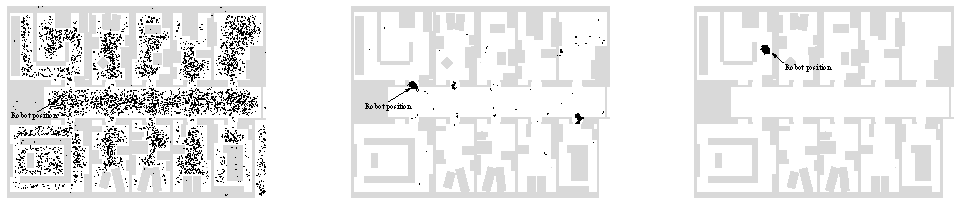
\includegraphics[width=\linewidth]{mcl_dieter_fox_example}

        \small
        Example of bi-modal distribution arising from the symmetry of the
        environment

        \source{http://www.aaai.org/Papers/AAAI/1999/AAAI99-050.pdf}{Fox et
        al., Monte Carlo Localization: Efficient Position Estimation for Mobile Robots}
    \end{center}
}
\end{frame}

\begin{frame}{Example: museum pose maintenance}

Monte Carlo using the ceiling of the Smithsonian museum

    \begin{center}
    \video{0.6\linewidth}{figs/part6/mcl.mp4}
    \end{center}

\end{frame}

\begin{frame}{Monte-Carlo Localisation -- Further reading}

    \begin{itemize}
        \item Thrun, Burgard, Fox, \emph{Probabilistic Robotics}
        \item Dellaert, Fox, Burgard, Thrun,
            \href{http://www.ri.cmu.edu/publication_view.html?pub_id=533}{Monte
            Carlo Localization for Mobile Robots}, \emph{IEEE International
            Conference on Robotics and Automation (ICRA99)}, May, 1999.

    \end{itemize}

    Videos of examples of MCL

    \begin{itemize}
        \item \url{http://www.youtube.com/watch?v=uU_1c_CxB1g}
        \item \url{http://www.youtube.com/watch?v=7K8dZwqBSSA}
        \item \url{https://www.youtube.com/watch?v=oKUYj1FWzN4}
        \item \url{https://www.youtube.com/watch?v=lCXv4yOcwf8}
    \end{itemize}

\end{frame}

\section{SLAM}


\begin{frame}{What is Simultaneous Localisation And Mapping?}

    Given an unknown environment and vehicle pose:

    \begin{itemize}
        \item Move through the environment
        \item Estimate the robot pose
        \item Generate a map of environmental features
    \end{itemize}

    \pause
    \begin{enumerate}
        \item Use the robot pose estimate to improve the map landmark position
            estimates

        \item Use the landmark estimates to improve the robot pose estimate

        \item Repeat
    \end{enumerate}
\end{frame}

\begin{frame}{Probabilistic Basis of SLAM}

    \begin{overprint}
    \onslide<1>
    Given:
    \begin{itemize}
        \item Robot control signal $u_k$ (or measurement $\rightarrow$ odometry)
        \item A set of feature observations $z_k$ (sensor measurements)
    \end{itemize}

    Estimate:

    \begin{itemize}
        \item Map of landmarks $M_{k+1}$
        \item Robot Pose $V_{k+1}$
    \end{itemize}

    Sources of Error:

    \begin{itemize}
        \item Control signal
        \item Motion model
        \item Sensor model
    \end{itemize}

    \onslide<2>
        \vspace{3em}

        \Large
        \[
            p(V_{k+1}, M_{k+1} | z_k, u_k)
        \]

        \normalsize

        \vspace{2em}

        $\Rightarrow$ estimate the joint probability of $V_{k+1}$ and $M_{k+1}$ conditioned on
        $z_k$ and $u_k$.

    \onslide<3->

        \vspace{3em}
        \large
        \begin{align*}
            p&(V_{k+1}, M_{k+1} | z_k, u_k) = \\
            &\eta \highlight<6>{p(z_{k+1} |\bubblemark[0pt]{sensormod} V_{k+1}, M_{k+1})} \int \highlight<5>{p(V_{k+1} |\bubblemark[0pt]{motionmod} V_k, u_k)} \highlight<4>{p(V_k, M_k |\bubblemark[0pt]{prior} z_k, u_k)} \mathrm{d} v_k
        \end{align*}

        \bubble<4>[90][0.5][4cm]{prior}{Prior state and covariance estimates from the last filter iteration}
        \bubble<5>[90][0.5][6cm]{motionmod}{Probabilistic motion model estimates the new
        vehicle pose covariance estimates from the prior estimate and the
        control}
        \bubble<6>[90][0.5][4cm]{sensormod}{Measurement model gives the expected value of the feature observations}
    \end{overprint}

\source{http://www.computerrobotvision.org/2010/slam_camp/collier_intro.pdf}{Jack Collier}

\end{frame}

\begin{frame}{SLAM families}

    \begin{itemize}
        \item \emph{Kalman filtering}: \textbf{Extended KF (EKF) SLAM} + a few others
        \item \emph{particle filtering}: Rao-Blackwellized particle filter
            (\textbf{FastSLAM})
    \end{itemize}
\end{frame}

\begin{frame}{Why is SLAM hard?}

\only<1>{
    \textbf{Chicken and egg problem}

If there is no map, how the robot localise itself. If the robot
  doesn't know its location, how can it build up a map?

Odometry is not to be trusted:

    \begin{center}
        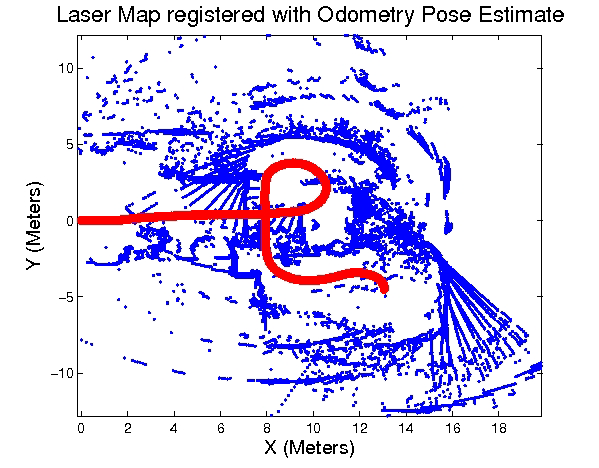
\includegraphics[width=0.4\linewidth]{slam1}
        \hspace{1em}
        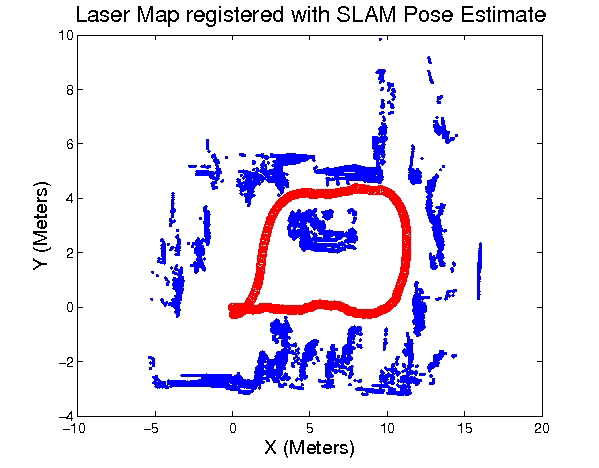
\includegraphics[width=0.4\linewidth]{slam2}
    \end{center}

}
    \only<2>{

        \textbf{Loop closure}

        \begin{columns}
            \begin{column}{0.5\linewidth}

                    \begin{itemize}
                        \item Even with the best SLAM algorithm, pose
                            uncertainty will increase as the vehicle moves
                        \item This pose uncertainty means that landmark
                            locations further from the map origin have a higher
                            uncertainty
                        \item \textbf{Revisiting a previously observed landmarks
                            significantly reduces uncertainty in robot and
                            landmark pose estimates}
                    \end{itemize}

            \end{column}
            \begin{column}{0.5\linewidth}
                \begin{center}
                    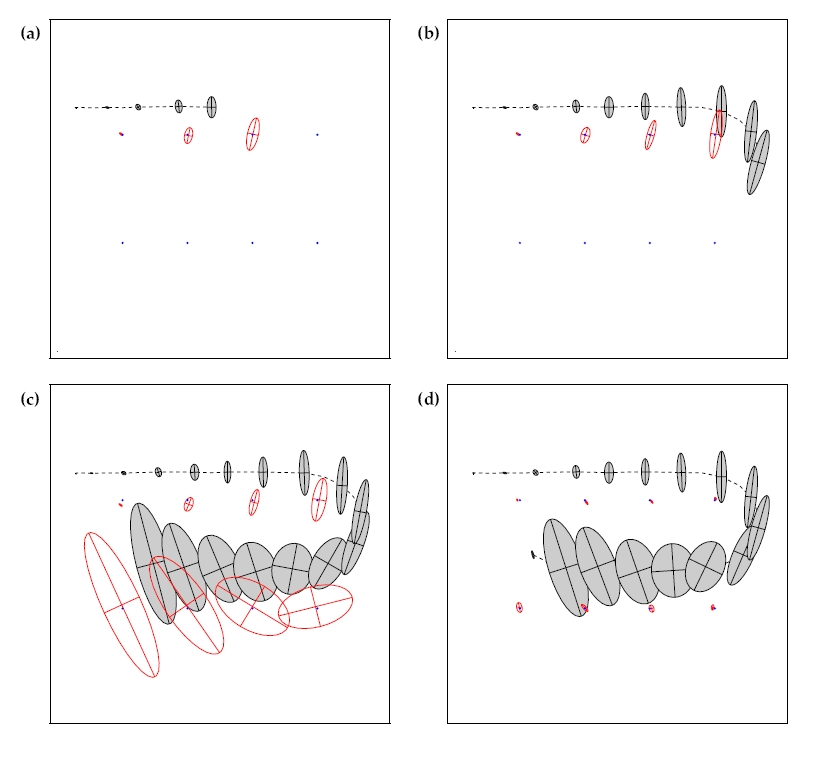
\includegraphics[width=\linewidth]{loopclosure}
                \end{center}
            \end{column}
        \end{columns}
    }

\source{http://www.computerrobotvision.org/2010/slam_camp/collier_intro.pdf}{Jack Collier}
\end{frame}

\begin{frame}[plain]

    \begin{center}
    \video[1.0]{0.7\linewidth}{figs/part6/slam.mp4}

    \source{http://youtu.be/Q1ipn42rMh8}{Robert Sim, University of British Columbia}
    \end{center}

\end{frame}

\imageframe{mapping_pepper}

\videoframe[0.56]{figs/part6/samsung_slam_vacuum.mp4}

\begin{frame}{SLAM -- Further reading}

    \begin{itemize}
        \item Take a MSc Robotics next year!
        \item \href{http://www.computerrobotvision.org/2010/slam_camp/collier_intro.pdf}{Jack
            Collier introduction (!!) to SLAM}
        \item Thrun, Burgard, Fox, \emph{Probabilistic Robotics}
    \end{itemize}
\end{frame}

\section{Path planning}

\begin{frame}{Metric vs topological maps}

    \begin{columns}
        \begin{column}{0.5\linewidth}

            \begin{center}
                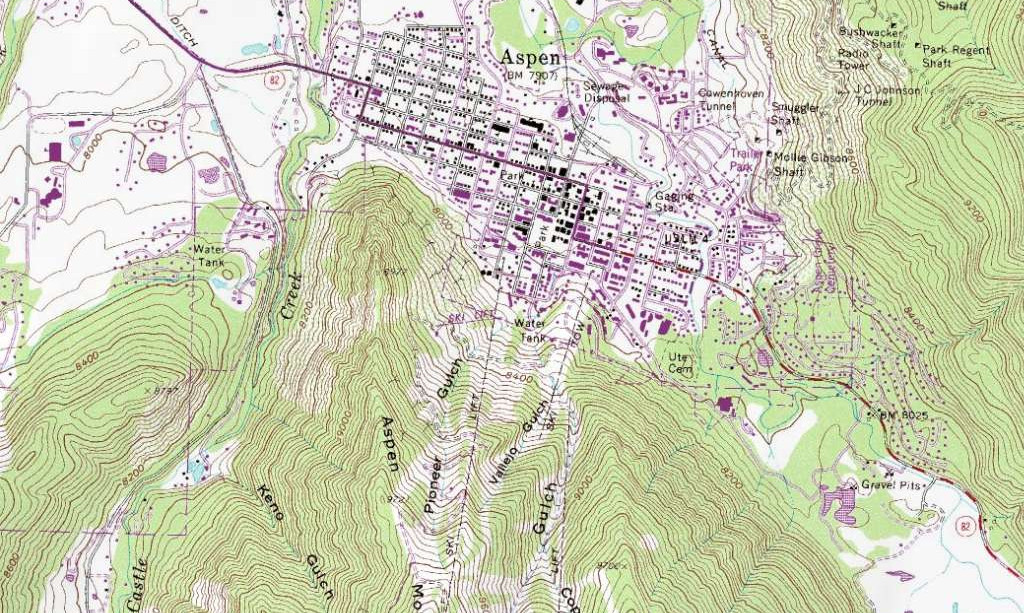
\includegraphics[width=0.8\linewidth]{map}
            \end{center}

            \small
            A metric map considers a two-dimensional space in which it places objects. The
            objects are placed with precise coordinates.

            This representation is convenient and natural, but \emph{sensitive to noise}
            and \emph{difficult to calculate the distances precisely}.

        \end{column}
        \begin{column}{0.5\linewidth}

            \begin{center}
                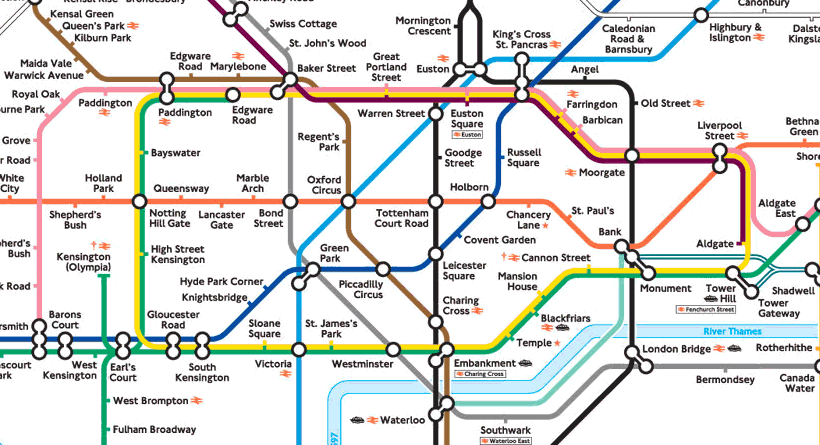
\includegraphics[width=0.8\linewidth]{tubemap}
            \end{center}

            \small
            A topological map only considers places and
            relations between them. Often, the distances between places
            are stored.

            The map is typically a \textbf{graph}, in which the nodes
            corresponds to places and edges correspond to the paths.
        \end{column}
    \end{columns}

    \normalsize

    \pause
    \textbf{Cell decomposition} can be used to transform a metric map into a
    topological one. More on that in a moment.

\end{frame}

\imageframe{topo-metric}
\imageframe{tubemap-2}

\begin{frame}{Path Planning: Configuration Space}

     The state or configuration $q$ of a robot can be described with $k$ values $q_i$.
        For example, for a two-link planar robot, $\theta_1$ and $\theta_2$:

        \begin{center}
        \resizebox{0.9\linewidth}{!}{
        \begin{tikzpicture}[>=latex]
            \only<1>{
            \node at (0,0){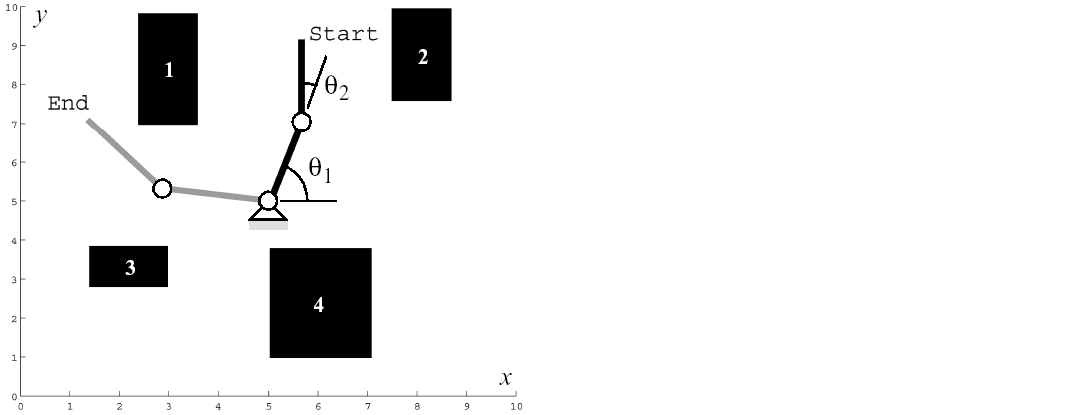
\includegraphics[width=\linewidth]{configurationspace0}};
            }
            \only<2->{
            \node at (0,0) {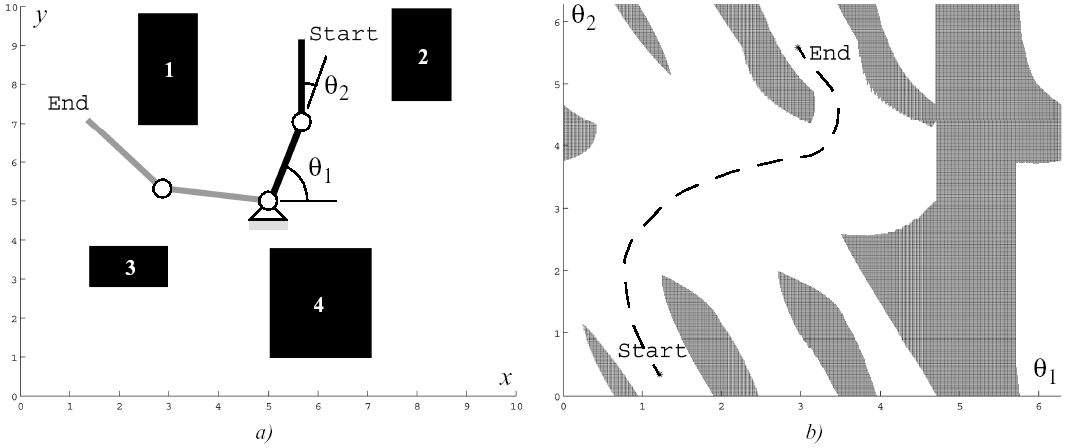
\includegraphics[width=\linewidth]{configurationspace}};

            \draw[thick,->] (5.5,-1) -- (4,-0.7) node[at start,
            right,align=left] {\footnotesize these regions\\\footnotesize correspond \\ \footnotesize to colliding $(\theta_1,\theta_2)$};
            \draw[thick,->] (5.5,-1) -- (3,-1.2);
            }
        \end{tikzpicture}
    }
        \end{center}

\onslide<2->
    Each $q$ is a point in a $k$-dimensional space called the
    \textbf{configuration space} $C$ of the robot.

    \onslide<3>
    We can map as well obstacles to \emph{configuration space obstacles} $O$.

    The \emph{free space} (where the robot is safe to move) is then $F = C - O$.

\end{frame}

\begin{frame}{Global vs local path planning}

        \begin{tikzpicture}[>=latex]
            \node at (0,0) {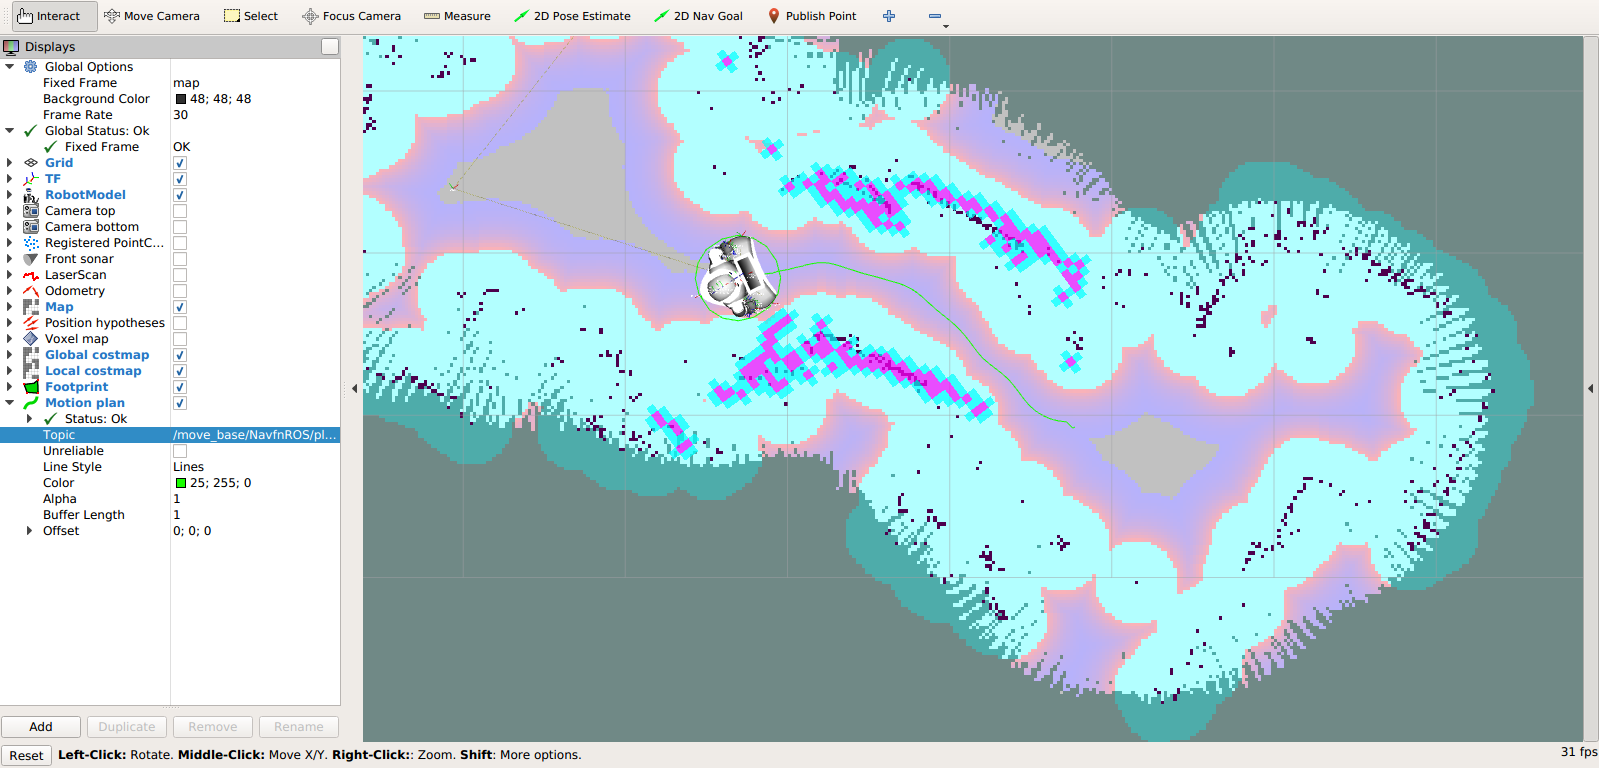
\includegraphics[width=\linewidth]{motion_planning_pepper_rviz}};

            \only<2>{
            \draw[thick,->] (-1,-1) -- (0,0) node[at start, below] {local costmap};
            \draw[thick,->] (0.3,-1.8) -- (2,-0.7) node[at start, below] {global costmap};
            \draw[thick,->] (0.3,-1.8) -- (1.9,-1);
            }
        \end{tikzpicture}

    \begin{columns}
        \begin{column}{0.5\linewidth}
            \textbf{Global path planning}

            \only<1>{
            \begin{itemize}
                \item long distances (\ie large map, slower calculations)
                \item static environment
            \end{itemize}
            }
            \only<2> {
                \vspace{1em}
                $\rightarrow$ global (static) \textbf{costmap}
            }
        \end{column}
        \begin{column}{0.5\linewidth}
            \textbf{Local path planning}

            \only<1>{
            \begin{itemize}
                \item short horizon
                \item dynamic environment (use of sensors)
            \end{itemize}
            }
            \only<2> {
                \vspace{1em}
                $\rightarrow$ local (dynamic) \textbf{costmap}
            }
        \end{column}
    \end{columns}

\end{frame}

\begin{frame}{Global path planning}

\emph{Assumptions}:

\begin{itemize}
\item A good enough map of the environment is available for navigation
  (topological or metric or a mixture between both).
\item The robot knows where it is on the map (using for example GPS or Monte
  Carlo localisation).
\end{itemize}

\pause

\emph{First step}: Build a representation of the environment using a \textbf{road-map (graph)},
        \textbf{cells} or a \textbf{potential field}. The resulting
        \emph{discrete} locations or cells allow then to use standard planning algorithms.

Possible algorithms:

\begin{itemize}
\item Visibility graph
\item Voronoi diagram
\item Cell decomposition $\rightarrow$ connectivity graph
\item Potential field
\end{itemize}

\end{frame}


\begin{frame}{Graphs: Visibility Graph}


    \begin{center}
        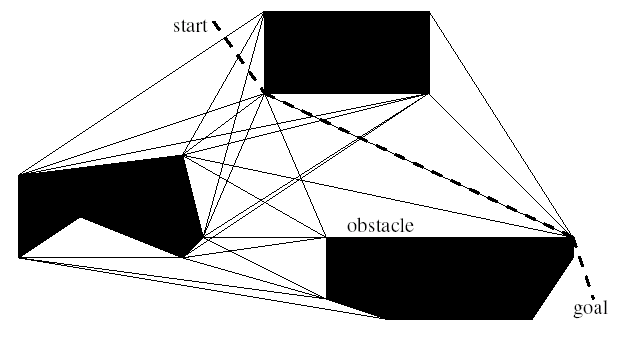
\includegraphics[width=\linewidth]{visibilitygraph}
    \end{center}

    Edges between nodes are the lines of sight from each corner to an
    obstacle to every other visible corner.

\end{frame}

\begin{frame}{Graphs: Voronoi graphs}

    \href{http://alexbeutel.com/webgl/voronoi.html}{Voronoi graph}: distance to obstacles from every nodes is maximal.

    \begin{center}
        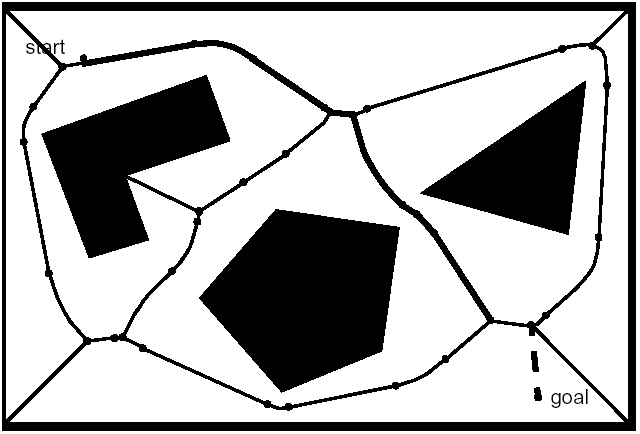
\includegraphics[width=0.7\linewidth]{voronoi}
    \end{center}

    (by moving along the edges of a Voronoi graph, the robot ensures it is
    always as far as possible from obstacles)

\end{frame}

\begin{frame}{Graphs: Cell Decomposition}

    \only<1>{
    Divide space into simple, connected regions called \textbf{cells}.

    Determine which open cells are adjacent and construct a \textbf{connectivity
    graph}.

    Find cells in which the initial and goal configuration (state) lie and
    search for a path in the connectivity graph to join them.

    From the sequence of cells found with an appropriate search algorithm,
    compute a path within each cell.

    \small
        \eg passing through the midpoints of cell boundaries or by sequence
            of wall following movements.

    }
    \only<2>{

    Example: exact cell decomposition

    \begin{center}
        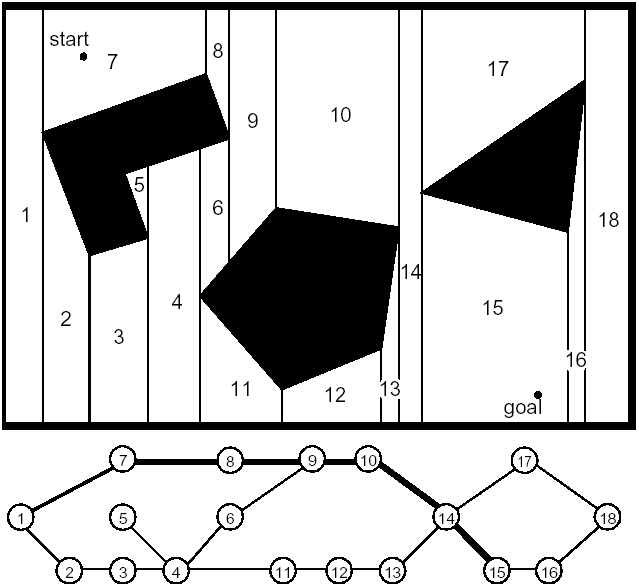
\includegraphics[width=0.6\linewidth]{exactcelldecomposition}
    \end{center}

    }
    \only<3>{

    Example: approximate cell decomposition

    \begin{center}
        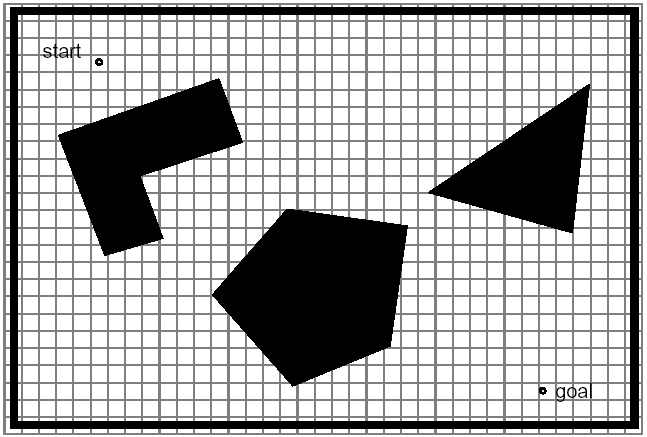
\includegraphics[width=0.5\linewidth]{celldecomposition1}
        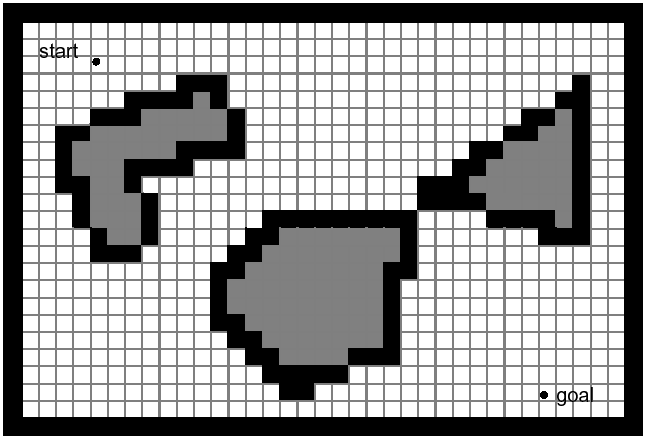
\includegraphics[width=0.5\linewidth]{celldecomposition2}
    \end{center}

    }
    \only<4>{

    Adaptive cell decomposition: changes the size of each cell according
    to the detail needed.

    \begin{center}
        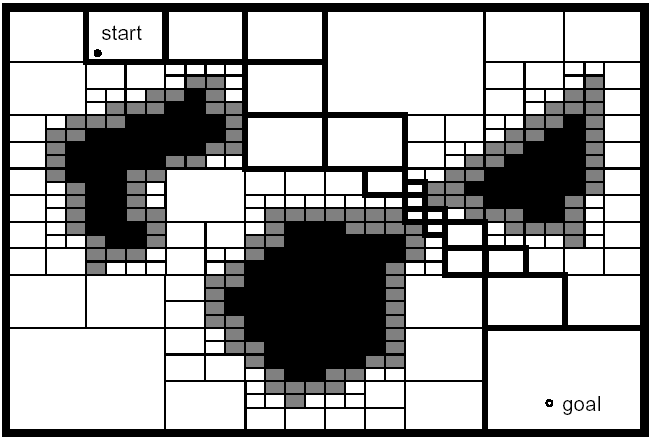
\includegraphics[width=0.8\linewidth]{adaptivecelldecomposition}
    \end{center}
}
\end{frame}

\begin{frame}{Representing graphs}

\begin{itemize}
\item How is a graph represented in a computer? Graphical representation is
  intuitive, but not straightforward to implement in a program.
\item Graphs can be represented as a matrix:
\end{itemize}

    \begin{columns}
        \begin{column}{0.5\linewidth}

    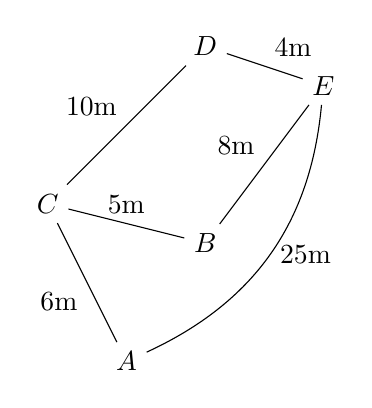
\begin{tikzpicture}[every edge quotes/.style={auto=right}]
        \node at (0,0) (A) {$A$};
        \node at (1,1.5) (B) {$B$};
        \node at (-1,2) (C) {$C$} edge["6m",left] (A)
                                 edge node[above] {5m} (B);
        \node at (1,4) (D) {$D$} edge["10m"] (C);
        \node at (2.5,3.5) (E) {$E$} edge["4m"] (D)
                                     edge["8m"] (B)
                                     edge[bend left] node[right] {25m} (A);

        %\draw (A) --[label=25m] (E) --[label=4m] (D) --[label=10m] (B) --[label=5m] (C) --[label=6m] (A);
        %\draw (E) --[label=8m] (B);
    \end{tikzpicture}
        \end{column}
        \begin{column}{0.5\linewidth}
            \begin{tabular}{llllll}
                           & \textbf{A} & \textbf{B} & \textbf{C} & \textbf{D} &
                           \textbf{E} \\
                           \textbf{A} & 0          & -          & 6          & -
                           & 25         \\
                           \textbf{B} & -          & 0          & 5          & -
                           & 8          \\
                           \textbf{C} & 6          & 5          & 0          &
                           10         & -          \\
                           \textbf{D} & -          & -          & 10         & 0
                           & 4          \\
                           \textbf{E} & 25         & 8          & -          & 4
                           & 0         
            \end{tabular}
        \end{column}
    \end{columns}

\end{frame}

\begin{frame}{Searching graphs}

Graphs can be searched, for example to find the shortest path between
two nodes.

Many different search algorithms exist

\begin{itemize}
\item \href{http://en.wikipedia.org/wiki/Breadth-first_search}{Breadth
  first}
\item \href{http://en.wikipedia.org/wiki/Depth-first_search}{Depth first}
\item \href{http://en.wikipedia.org/wiki/A*_search_algorithm}{A*}
\item \href{http://en.wikipedia.org/wiki/Dijkstra's_algorithm}{Dijkstra's
  shortest path}
\end{itemize}

\end{frame}

\begin{frame}{Dijkstra's algorithm: illustration}

    \begin{center}
        \video[1]{0.4\linewidth}{figs/part6/dijkstra.mp4}

        \source{http://en.wikipedia.org/wiki/Dijkstra's_algorithm}{Wikipedia}
    \end{center}

    Dijkstra search between start (red) and goal (green)
    positions.

    Note how Dijkstra is expanding its search out from the
    starting position, without knowledge about which nodes could bring it
    closer to the goal.

\end{frame}

\begin{frame}[fragile]{Searching graphs - Dijkstra}

\begin{pythoncode*}{frame=none,escapeinside=||}
def dijkstra(graph, weights, start_node):

  dist = {} # maps nodes to distance to 'start_node'
  previous = {} # needed to reconstruct shortest path

  for node in graph:
    dist[node] = math.inf # initial dist. from 'start_node' to 'node'

  dist[start_node] = 0

  Q = graph.nodes() # unvisited nodes
  while not Q.empty():
    u = pop_min(Q) # remove best node

    for v in u.neighbours: # iterate over nodes connected to u
      if dist[u] + weights(u, v) < dist[v]: # new shorter path to v!
        dist[v] = dist[u] + weights(u, v)
        previous[v] = u

  return dist, previous
\end{pythoncode*}
\end{frame}


\begin{frame}[fragile]{Searching graphs -- Dijkstra}

    Reading out shortest path from the start node to goal \python{end_node}:

\begin{pythoncode}
path = []
node = end_node # goal
while node in previous:
path = [node] + path # append at the front of our path
node = previous[node]
\end{pythoncode}

    Returns the shortest path (if there are more than one, only one is returned).

    Returns empty if no path exists.

\end{frame}

\begin{frame}{The cost of search}

Maps can be huge

\begin{itemize}
    \item For example, 10,000 $m^2$ shopping mall ($\sim$ Marshmills' Sainsburys), with a 10x10cm map
    resolution, requires $10^{10}$ = 10 billion nodes on the graph!
\end{itemize}

Search time can be problematic:

\begin{itemize}
\item Dijkstra has a complexity of $O(N+V^2)$. For example, for a map with
    $10^7$ nodes and $10^8$ vertices, it can take $10^7+10^{2\times 8} \sim
        10^{16}$ calculations to
  find a shortest path between two points.
\item Some implementations are much more efficient. A* search is at worst
  the same as Dijkstra, but can be polynomial in the number of nodes
  $O(N^k)$ when a good heuristic is used. For example, if you can
  choose between two nodes to explore, take the node closer to the goal.
\end{itemize}

\end{frame}

\begin{frame}{A* algorithm - illustration}

    \begin{center}
        \video[1]{0.4\linewidth}{figs/part6/astar.mp4}

        \source{http://en.wikipedia.org/wiki/A*_search_algorithm}{Wikipedia}
    \end{center}

    A* search for finding path between start and goal position.

    A* uses a \textbf{heuristic} (here the distance to the goal) to guide the
    exploration (first expand to nodes closer to the goal). This gives a chance of finding
    the solution in less time.

\end{frame}

\section{Potential field path planning}

\begin{frame}{Potential Field Path Planning}

    \only<1>{
        Robot is treated as a \emph{point under the influence} of an artificial
    potential field.

    \begin{itemize}
        \item Generated robot movement is similar to a ball rolling down the hill
        \item Goal generates attractive force
        \item Obstacle are repulsive forces
    \end{itemize}

    Needed:

    \begin{itemize}
        \item Location of robot
        \item Location of obstacles
        \item $\Rightarrow$ a metric map is well suited
    \end{itemize}

    }
    \only<2>{

        \begin{center}
            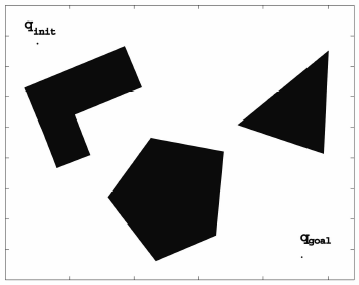
\includegraphics[width=0.4\linewidth]{potentialfields1}
            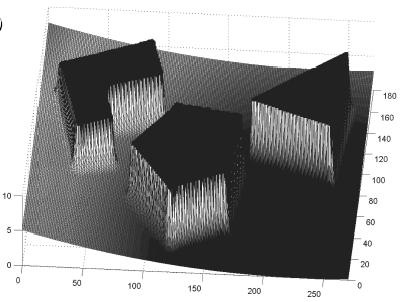
\includegraphics[width=0.4\linewidth]{potentialfields3}

            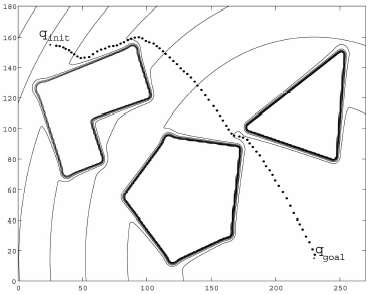
\includegraphics[width=0.4\linewidth]{potentialfields2}
        \end{center}

    }
\end{frame}

\begin{frame}{Potential field generation}

    Generation of potential field function $U(q)$

    \begin{itemize}
        \item attracting (goal) and repulsing (obstacle) fields
        \item summing up the fields
        \item functions must be
            \href{http://en.wikipedia.org/wiki/Differentiable_function}{differentiable}
    \end{itemize}

    \pause

    Generate artificial force field $F(q)$

    \[
        F(q) = -\nabla U(q) = -\nabla U_{att}(q) - \nabla U_{rep}(q) =
    \begin{bmatrix}\frac{\partial U}{x} \\ \frac{\partial U}{y}\end{bmatrix}
        \]

    \pause

    Set robot speed $(v_x, v_y)$ proportional to the force
    $F(q)$ generated by the field

    \begin{itemize}
        \item the force field drives the robot to the goal
        \item if robot is assumed to be a point mass
    \end{itemize}


\end{frame}

\begin{frame}{Potential Field Path Planning}

Attractive potential field

\begin{itemize}
\item For example, a parabolic function representing the Euclidean distance
    $\rho = || q - q_{goal} ||$ to the goal:

        \[
            U_{att}(q) = \frac{1}{2} k_{att} \cdot \rho_{goal}^2(q)
            \]

\item Attracting force converges linearly towards 0 (goal)

    \begin{align*}
        F_{att}(q) &= - \nabla U_{att}(q) \\
                &= -k_{att}\cdot \rho_{goal}(q) \nabla \rho_{goal}(q) \\
                &= -k_{att}\cdot (q - q_{goal})
    \end{align*}
\end{itemize}

\end{frame}

\begin{frame}{Potential Field Path Planning}

Repulsing potential field

Should generate a barrier around all the obstacle

\begin{itemize}
\item strong if close to the obstacle
\item no influence if far from the obstacle:
    \[
        U_{rep}(q) = \left\{\begin{matrix}
                            \frac{1}{2}k_{rep}(\frac{1}{\rho(q)} -
                            \frac{1}{\rho_0})^2 &  \text{if }
                            \rho(q)\bubblemark{rhoq} <  \rho_0 \\ 
                            0 & \text{if } \rho(q) \geq \rho_0 
                        \end{matrix}\right.
    \]
\item field is positive or zero and \emph{tends to infinity} as q gets
  closer to the object:
    \[
        F_{rep}(q) = -\nabla U_{rep}(q) = \left\{\begin{matrix}
            k_{rep}(\frac{1}{\rho(q)} - \frac{1}{\rho_0}) \cdot \frac{1}{\rho(q)^2} &  \text{if }  \rho(q) <  \rho_0 \\ 
                                              0 & \text{if } \rho(q) \geq \rho_0 
                                          \end{matrix}\right.
    \]
\end{itemize}

    \bubble<1>{rhoq}{distance to obstacle}
\end{frame}

\begin{frame}{Potential Field Path Planning}

    Notes:

    \begin{itemize}
        \item \textbf{Local minima problem} exists: robot can get stuck in places on the map
            where the potential field has a local dip.
        \item problem is getting more complex if the robot is not considered as a
            point mass
        \item If objects are convex there exists situations where several minimal
            distances exist $\rightarrow$ can result in oscillations
        \item Robot path oscillates, \eg in narrow passages.
    \end{itemize}


    Videos:

    \begin{itemize}
        \item \url{http://www.youtube.com/watch?v=DxzRYYMjxKY}
        \item \url{http://www.youtube.com/watch?v=JnPfu7xHNt4}
    \end{itemize}

\end{frame}

\begin{frame}{Extended Potential Field Path Planning}

    Additionally a \textbf{rotation potential field} and a \textbf{task
    potential field} are introduced.

    \vspace{1em}

    \begin{columns}
        \begin{column}{0.5\linewidth}

            \textbf{Rotation potential field}

            \begin{itemize}
                \item force is also a function of robots orientation to the obstacle
            \end{itemize}

            \textbf{Task potential field}

            \begin{itemize}
                \item filters out the obstacles that should not influence the robots
                    movements, \ie only the obstacles in front of the robot are considered
            \end{itemize}

        \end{column}
        \begin{column}{0.5\linewidth}
            \begin{center}
                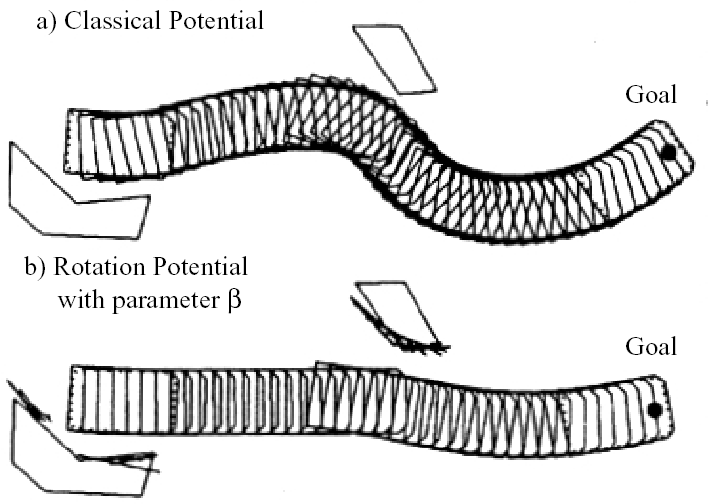
\includegraphics[width=\linewidth]{potentialfield}
            \end{center}
        \end{column}
    \end{columns}

\end{frame}

\section{Grassfire algorithm}

\begin{frame}{Grassfire algorithm}

\begin{itemize}
    \item Starting from a metric map, a \textbf{wave front} is expanded around the goal.
\item Goal is reached by travelling on descending values.
\end{itemize}

    \begin{center}
        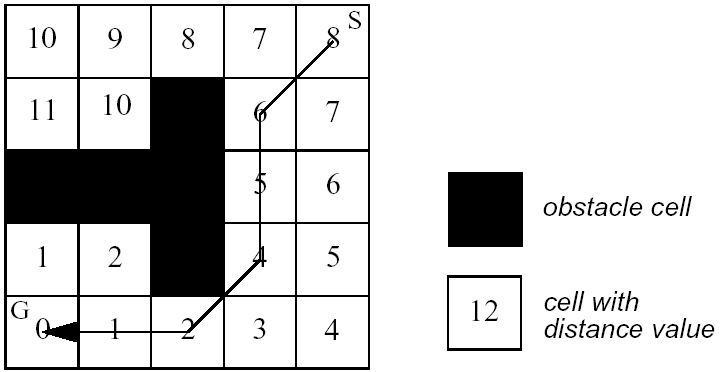
\includegraphics[width=0.7\linewidth]{grassfire}
    \end{center}
\end{frame}

\begin{frame}{Grassfire algorithm}
    \begin{center}
        \only<1>{
            \begin{tabular}{rcccccccccccc}
                \textbf{}                        & \multicolumn{1}{l}{\textbf{A}} & \multicolumn{1}{l}{\textbf{B}}                 & \multicolumn{1}{l}{\textbf{C}}                & \multicolumn{1}{l}{\textbf{D}}                & \multicolumn{1}{l}{\textbf{E}}                & \multicolumn{1}{l}{\textbf{F}} & \multicolumn{1}{l}{\textbf{G}} & \multicolumn{1}{l}{\textbf{H}}                 & \multicolumn{1}{l}{\textbf{I}}                & \multicolumn{1}{l}{\textbf{J}}                & \multicolumn{1}{l}{\textbf{K}}                & \multicolumn{1}{l}{\textbf{L}} \\ \cline{2-13} 
                \multicolumn{1}{r|}{\textbf{1}}  & \multicolumn{1}{c|}{}          & \multicolumn{1}{c|}{}                          & \multicolumn{1}{c|}{}                         & \multicolumn{1}{c|}{}                         & \multicolumn{1}{c|}{}                         & \multicolumn{1}{c|}{}          & \multicolumn{1}{c|}{}          & \multicolumn{1}{c|}{}                          & \multicolumn{1}{c|}{}                         & \multicolumn{1}{c|}{}                         & \multicolumn{1}{c|}{}                         & \multicolumn{1}{c|}{}          \\ \cline{2-13} 
                \multicolumn{1}{r|}{\textbf{2}}  & \multicolumn{1}{c|}{}          & \multicolumn{1}{c|}{}                          & \multicolumn{1}{c|}{}                         & \multicolumn{1}{c|}{}                         & \multicolumn{1}{c|}{}                         & \multicolumn{1}{c|}{}          & \multicolumn{1}{c|}{}          & \multicolumn{1}{c|}{\cellcolor[HTML]{000000}}  & \multicolumn{1}{c|}{\cellcolor[HTML]{000000}} & \multicolumn{1}{c|}{\cellcolor[HTML]{000000}} & \multicolumn{1}{c|}{\cellcolor[HTML]{000000}} & \multicolumn{1}{c|}{}          \\ \cline{2-13} 
                \multicolumn{1}{r|}{\textbf{3}}  & \multicolumn{1}{c|}{}          & \multicolumn{1}{c|}{}                          & \multicolumn{1}{c|}{}                         & \multicolumn{1}{c|}{}                         & \multicolumn{1}{c|}{}                         & \multicolumn{1}{c|}{}          & \multicolumn{1}{c|}{}          & \multicolumn{1}{c|}{}                          & \multicolumn{1}{c|}{}                         & \multicolumn{1}{c|}{}                         & \multicolumn{1}{c|}{}                         & \multicolumn{1}{c|}{}          \\ \cline{2-13} 
                \multicolumn{1}{r|}{\textbf{4}}  & \multicolumn{1}{c|}{}          & \multicolumn{1}{c|}{}                          & \multicolumn{1}{c|}{}                         & \multicolumn{1}{c|}{}                         & \multicolumn{1}{c|}{}                         & \multicolumn{1}{c|}{}          & \multicolumn{1}{c|}{}          & \multicolumn{1}{c|}{}                          & \multicolumn{1}{c|}{}                         & \multicolumn{1}{c|}{}                         & \multicolumn{1}{c|}{}                         & \multicolumn{1}{c|}{}          \\ \cline{2-13} 
                \multicolumn{1}{r|}{\textbf{5}}  & \multicolumn{1}{c|}{}          & \multicolumn{1}{c|}{\cellcolor[HTML]{63AC4B}S} & \multicolumn{1}{c|}{}                         & \multicolumn{1}{c|}{\cellcolor[HTML]{000000}} & \multicolumn{1}{c|}{\cellcolor[HTML]{000000}} & \multicolumn{1}{c|}{}          & \multicolumn{1}{c|}{}          & \multicolumn{1}{c|}{}                          & \multicolumn{1}{c|}{}                         & \multicolumn{1}{c|}{}                         & \multicolumn{1}{c|}{}                         & \multicolumn{1}{c|}{}          \\ \cline{2-13} 
                \multicolumn{1}{r|}{\textbf{6}}  & \multicolumn{1}{c|}{}          & \multicolumn{1}{c|}{}                          & \multicolumn{1}{c|}{}                         & \multicolumn{1}{c|}{}                         & \multicolumn{1}{c|}{\cellcolor[HTML]{000000}} & \multicolumn{1}{c|}{}          & \multicolumn{1}{c|}{}          & \multicolumn{1}{c|}{}                          & \multicolumn{1}{c|}{}                         & \multicolumn{1}{c|}{\cellcolor[HTML]{000000}} & \multicolumn{1}{c|}{}                         & \multicolumn{1}{c|}{}          \\ \cline{2-13} 
                \multicolumn{1}{r|}{\textbf{7}}  & \multicolumn{1}{c|}{}          & \multicolumn{1}{c|}{}                          & \multicolumn{1}{c|}{}                         & \multicolumn{1}{c|}{}                         & \multicolumn{1}{c|}{\cellcolor[HTML]{000000}} & \multicolumn{1}{c|}{}          & \multicolumn{1}{c|}{}          & \multicolumn{1}{c|}{\cellcolor[HTML]{CA4444}G} & \multicolumn{1}{c|}{}                         & \multicolumn{1}{c|}{\cellcolor[HTML]{000000}} & \multicolumn{1}{c|}{}                         & \multicolumn{1}{c|}{}          \\ \cline{2-13} 
                \multicolumn{1}{r|}{\textbf{8}}  & \multicolumn{1}{c|}{}          & \multicolumn{1}{c|}{}                          & \multicolumn{1}{c|}{\cellcolor[HTML]{000000}} & \multicolumn{1}{c|}{\cellcolor[HTML]{000000}} & \multicolumn{1}{c|}{\cellcolor[HTML]{000000}} & \multicolumn{1}{c|}{}          & \multicolumn{1}{c|}{}          & \multicolumn{1}{c|}{}                          & \multicolumn{1}{c|}{}                         & \multicolumn{1}{c|}{\cellcolor[HTML]{000000}} & \multicolumn{1}{c|}{}                         & \multicolumn{1}{c|}{}          \\ \cline{2-13} 
                \multicolumn{1}{r|}{\textbf{9}}  & \multicolumn{1}{c|}{}          & \multicolumn{1}{c|}{}                          & \multicolumn{1}{c|}{}                         & \multicolumn{1}{c|}{}                         & \multicolumn{1}{c|}{}                         & \multicolumn{1}{c|}{}          & \multicolumn{1}{c|}{}          & \multicolumn{1}{c|}{}                          & \multicolumn{1}{c|}{}                         & \multicolumn{1}{c|}{\cellcolor[HTML]{000000}} & \multicolumn{1}{c|}{}                         & \multicolumn{1}{c|}{}          \\ \cline{2-13} 
                \multicolumn{1}{r|}{\textbf{10}} & \multicolumn{1}{c|}{}          & \multicolumn{1}{c|}{}                          & \multicolumn{1}{c|}{}                         & \multicolumn{1}{c|}{}                         & \multicolumn{1}{c|}{}                         & \multicolumn{1}{c|}{}          & \multicolumn{1}{c|}{}          & \multicolumn{1}{c|}{}                          & \multicolumn{1}{c|}{}                         & \multicolumn{1}{c|}{\cellcolor[HTML]{000000}} & \multicolumn{1}{c|}{}                         & \multicolumn{1}{c|}{}          \\ \cline{2-13} 
            \end{tabular}
        }
        \only<2>{

            \begin{tabular}{rcccccccccccc}
                \textbf{}                        & \multicolumn{1}{l}{\textbf{A}} & \multicolumn{1}{l}{\textbf{B}}                 & \multicolumn{1}{l}{\textbf{C}}                 & \multicolumn{1}{l}{\textbf{D}}                 & \multicolumn{1}{l}{\textbf{E}}                 & \multicolumn{1}{l}{\textbf{F}}                 & \multicolumn{1}{l}{\textbf{G}}                 & \multicolumn{1}{l}{\textbf{H}}                 & \multicolumn{1}{l}{\textbf{I}}                & \multicolumn{1}{l}{\textbf{J}}                & \multicolumn{1}{l}{\textbf{K}}                & \multicolumn{1}{l}{\textbf{L}} \\ \cline{2-13} 
                \multicolumn{1}{r|}{\textbf{1}}  & \multicolumn{1}{c|}{13}        & \multicolumn{1}{c|}{12}                        & \multicolumn{1}{c|}{11}                        & \multicolumn{1}{c|}{10}                        & \multicolumn{1}{c|}{9}                         & \multicolumn{1}{c|}{8}                         & \multicolumn{1}{c|}{7}                         & \multicolumn{1}{c|}{8}                         & \multicolumn{1}{c|}{9}                        & \multicolumn{1}{c|}{10}                       & \multicolumn{1}{c|}{11}                       & \multicolumn{1}{c|}{10}        \\ \cline{2-13} 
                \multicolumn{1}{r|}{\textbf{2}}  & \multicolumn{1}{c|}{12}        & \multicolumn{1}{c|}{11}                        & \multicolumn{1}{c|}{10}                        & \multicolumn{1}{c|}{9}                         & \multicolumn{1}{c|}{8}                         & \multicolumn{1}{c|}{7}                         & \multicolumn{1}{c|}{6}                         & \multicolumn{1}{c|}{\cellcolor[HTML]{000000}}  & \multicolumn{1}{c|}{\cellcolor[HTML]{000000}} & \multicolumn{1}{c|}{\cellcolor[HTML]{000000}} & \multicolumn{1}{c|}{\cellcolor[HTML]{000000}} & \multicolumn{1}{c|}{9}         \\ \cline{2-13} 
                \multicolumn{1}{r|}{\textbf{3}}  & \multicolumn{1}{c|}{11}        & \multicolumn{1}{c|}{10}                        & \multicolumn{1}{c|}{9}                         & \multicolumn{1}{c|}{8}                         & \multicolumn{1}{c|}{7}                         & \multicolumn{1}{c|}{6}                         & \multicolumn{1}{c|}{5}                         & \multicolumn{1}{c|}{4}                         & \multicolumn{1}{c|}{5}                        & \multicolumn{1}{c|}{6}                        & \multicolumn{1}{c|}{7}                        & \multicolumn{1}{c|}{8}         \\ \cline{2-13} 
                \multicolumn{1}{r|}{\textbf{4}}  & \multicolumn{1}{c|}{10}        & \multicolumn{1}{c|}{9}                         & \multicolumn{1}{c|}{\cellcolor[HTML]{FFCC67}8} & \multicolumn{1}{c|}{\cellcolor[HTML]{FFCC67}7} & \multicolumn{1}{c|}{\cellcolor[HTML]{FFCC67}6} & \multicolumn{1}{c|}{\cellcolor[HTML]{FFCC67}5} & \multicolumn{1}{c|}{4}                         & \multicolumn{1}{c|}{3}                         & \multicolumn{1}{c|}{4}                        & \multicolumn{1}{c|}{5}                        & \multicolumn{1}{c|}{6}                        & \multicolumn{1}{c|}{7}         \\ \cline{2-13} 
                \multicolumn{1}{r|}{\textbf{5}}  & \multicolumn{1}{c|}{11}        & \multicolumn{1}{c|}{\cellcolor[HTML]{63AC4B}S} & \multicolumn{1}{c|}{\cellcolor[HTML]{FFCC67}9} & \multicolumn{1}{c|}{\cellcolor[HTML]{000000}}  & \multicolumn{1}{c|}{\cellcolor[HTML]{000000}}  & \multicolumn{1}{c|}{\cellcolor[HTML]{FFCC67}4} & \multicolumn{1}{c|}{\cellcolor[HTML]{FFCC67}3} & \multicolumn{1}{c|}{2}                         & \multicolumn{1}{c|}{3}                        & \multicolumn{1}{c|}{4}                        & \multicolumn{1}{c|}{5}                        & \multicolumn{1}{c|}{6}         \\ \cline{2-13} 
                \multicolumn{1}{r|}{\textbf{6}}  & \multicolumn{1}{c|}{12}        & \multicolumn{1}{c|}{11}                        & \multicolumn{1}{c|}{10}                        & \multicolumn{1}{c|}{11}                        & \multicolumn{1}{c|}{\cellcolor[HTML]{000000}}  & \multicolumn{1}{c|}{3}                         & \multicolumn{1}{c|}{\cellcolor[HTML]{FFCC67}2} & \multicolumn{1}{c|}{\cellcolor[HTML]{FFCC67}1} & \multicolumn{1}{c|}{2}                        & \multicolumn{1}{c|}{\cellcolor[HTML]{000000}} & \multicolumn{1}{c|}{6}                        & \multicolumn{1}{c|}{7}         \\ \cline{2-13} 
                \multicolumn{1}{r|}{\textbf{7}}  & \multicolumn{1}{c|}{11}        & \multicolumn{1}{c|}{10}                        & \multicolumn{1}{c|}{11}                        & \multicolumn{1}{c|}{12}                        & \multicolumn{1}{c|}{\cellcolor[HTML]{000000}}  & \multicolumn{1}{c|}{2}                         & \multicolumn{1}{c|}{1}                         & \multicolumn{1}{c|}{\cellcolor[HTML]{CA4444}G} & \multicolumn{1}{c|}{1}                        & \multicolumn{1}{c|}{\cellcolor[HTML]{000000}} & \multicolumn{1}{c|}{7}                        & \multicolumn{1}{c|}{8}         \\ \cline{2-13} 
                \multicolumn{1}{r|}{\textbf{8}}  & \multicolumn{1}{c|}{10}        & \multicolumn{1}{c|}{9}                         & \multicolumn{1}{c|}{\cellcolor[HTML]{000000}}  & \multicolumn{1}{c|}{\cellcolor[HTML]{000000}}  & \multicolumn{1}{c|}{\cellcolor[HTML]{000000}}  & \multicolumn{1}{c|}{3}                         & \multicolumn{1}{c|}{2}                         & \multicolumn{1}{c|}{1}                         & \multicolumn{1}{c|}{2}                        & \multicolumn{1}{c|}{\cellcolor[HTML]{000000}} & \multicolumn{1}{c|}{8}                        & \multicolumn{1}{c|}{9}         \\ \cline{2-13} 
                \multicolumn{1}{r|}{\textbf{9}}  & \multicolumn{1}{c|}{9}         & \multicolumn{1}{c|}{8}                         & \multicolumn{1}{c|}{7}                         & \multicolumn{1}{c|}{6}                         & \multicolumn{1}{c|}{5}                         & \multicolumn{1}{c|}{4}                         & \multicolumn{1}{c|}{3}                         & \multicolumn{1}{c|}{2}                         & \multicolumn{1}{c|}{3}                        & \multicolumn{1}{c|}{\cellcolor[HTML]{000000}} & \multicolumn{1}{c|}{9}                        & \multicolumn{1}{c|}{10}        \\ \cline{2-13} 
                \multicolumn{1}{r|}{\textbf{10}} & \multicolumn{1}{c|}{10}        & \multicolumn{1}{c|}{9}                         & \multicolumn{1}{c|}{8}                         & \multicolumn{1}{c|}{7}                         & \multicolumn{1}{c|}{6}                         & \multicolumn{1}{c|}{5}                         & \multicolumn{1}{c|}{4}                         & \multicolumn{1}{c|}{3}                         & \multicolumn{1}{c|}{4}                        & \multicolumn{1}{c|}{\cellcolor[HTML]{000000}} & \multicolumn{1}{c|}{10}                       & \multicolumn{1}{c|}{11}        \\ \cline{2-13} 
            \end{tabular}
        }
    \end{center}

\end{frame}

\imageframe[scale=0.9]{grassfire2}

\begin{frame}[fragile]{Grassfire algorithm}

\begin{pythoncode}

def grassfire(M, goal):
    Q.push(goal)
    M[goal] = 0 # set goal value to 0

    while not Q.empty(): # loop until map filled
        a = Q.pop()

        for n in neighbours(a):
            if not n in M and not is_obstacle(n):
                Q.push(n)
                M[n] = M[a] + 1
    return M
\end{pythoncode}

Q is a \href{http://en.wikipedia.org/wiki/Queue_(abstract_data_type)}{queue
data structure}, a first-in first-out (fifo) list. The queue keeps track of
which locations on the map still need to be visited.

\end{frame}


\begin{frame}{}
    \begin{center}
        \Large
        That's all, folks!\\[2em]
        \normalsize
        Questions:\\
        Portland Square A216 or \url{severin.lemaignan@plymouth.ac.uk} \\[1em]

        Slides:\\ \href{https://github.com/severin-lemaignan/module-mobile-and-humanoid-robots}{\small github.com/severin-lemaignan/module-mobile-and-humanoid-robots}

    \end{center}
\end{frame}



\end{document}
